\newpage\subsection*{Άσκηση 4}

Το θεώρημα του \en{Koning} λέει ότι ((κάθε απλό γράφημα $G$ με μέγιστο βαθμό $\Delta(G)$ είναι 
επαγώμενο υπογράφημα κάποιου απλού $\Delta(G)$-κανονικού γραφήματος)) (για την απόδειξη 
δείτε σελ. 33 των σημειώσεων).

\begin{enumerate}[i.]
\item
Βρείτε πόσες επαναλήψεις χρειάζονται για την κατασκευή του $\Delta(G)$-κανονικού γραφήματος,
όπως περιγράφεται στην απόδειξη του θεωρήματος.

\item
Έστω ότι αναζητούμε απλό $\Delta(G)$-κανονικό γράφημα που να περιέχει το $G$ ως υπογράφημα 
(όχι απαραίτητα επαγώμενο). Είναι εφικτό μόνο με την προσθήκη ακμών στο $G$? Δώστε παράδειγμα 
με λίγες κορυφές στην περίπτωση του $\Delta(G)=3.4$.

\end{enumerate}

\subsubsection*{Λύση}

\begin{enumerate}[i.]

\item
Θα χρειαστούν $\Delta(G)-\delta(G)$ επαναλήψεις αφού σε κάθε επανάληψη κάθε κόμβος με βαθμό μικρότερο απο $\Delta(G)$ αυξάνεται κατά ένα.

\item
Δεν είναι πάντα εφικτό να βρούμε απλό $\Delta(G)$-κανονικό γράφημα που να περιέχει το $G$ ως υπογράφημα
μόνο με την προσθήκη ακμών στο $G$. Συγκεκριμένα, μπορούμε για κάθε αριθμό κόμβων να κατασκευάσουμε γράφο $G$
        που είναι ένωση ενός $(|V(G)|-1)$-κανονικού γράφου και ενός κόμβου μηδενικού βαθμού. Οποιαδήποτε προσθήκη ακμής σε αυτόν
τον γράφο θα δημιουργούσε κόμβο βαθμού μεγαλύτερου του $\Delta(G)$.

Σε συγκεκριμένες περιπτώσεις ωστόσο είναι εφικτό:

\begin{center}
    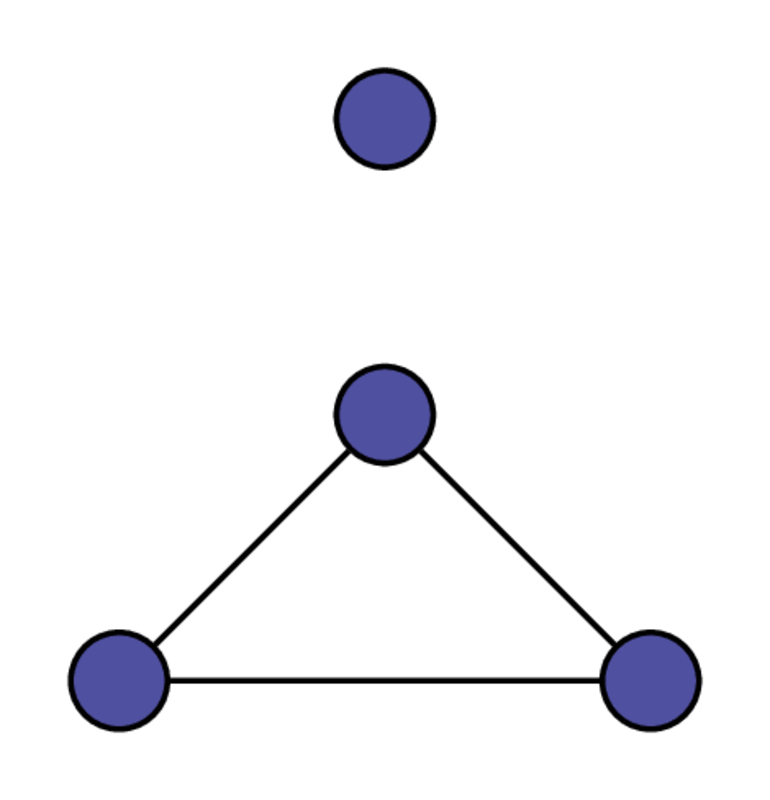
\includegraphics[width=.23\textwidth]{./exercise4/diagrams/d1.png} \hspace{3cm}
    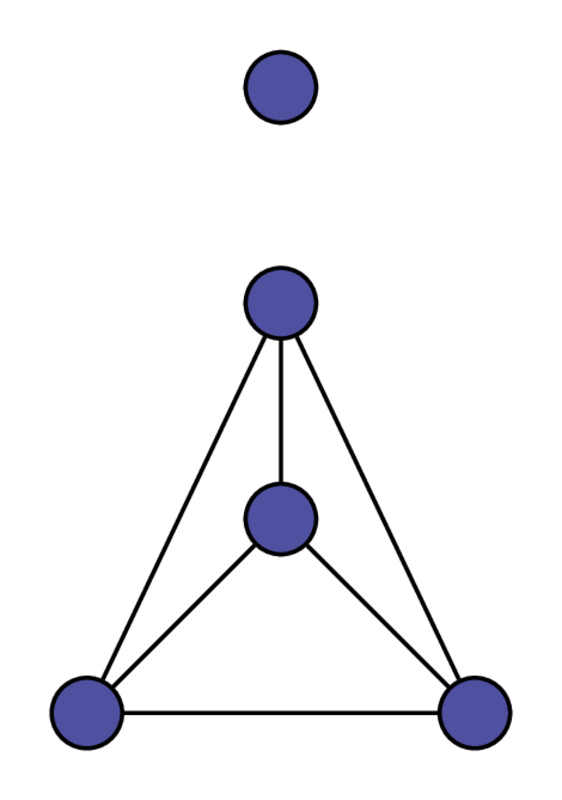
\includegraphics[width=.23\textwidth]{./exercise4/diagrams/d2.png} 
\end{center}

\end{enumerate}


